\documentclass[a4paper,12pt]{article}
%\documentclass[a4paper,12pt]{scrartcl}

\usepackage{xltxtra}

\input{../preamble.tex}

% \usepackage[spanish]{babel}

% \setromanfont[Mapping=tex-text]{Linux Libertine O}
% \setsansfont[Mapping=tex-text]{DejaVu Sans}
% \setmonofont[Mapping=tex-text]{DejaVu Sans Mono}

\title{Exam \#2}
\author{Isaac Ayala Lozano}
\date{\today}

\begin{document}
\maketitle

\section{Introduction}

The results of a Bayesian multivariate classifier are presented.
An explanation of its development is provided.
The classifier was trained to work with three categories $C_i$ and a
feature vector of size 2.

The classifier was trained using the Iris flower data set
\cite{fisher1936iris}, available from the UCI Machine
Learning Repository \footnote{https://archive.ics.uci.edu/ml/datasets/Iris}.
The dataset describes five properties of three different flower species:
petal length, petal width, sepal length, sepal width and variety.
Whilst the first four are quantitative traits, the last one is qualitative.
This trait describes the type flower associated with the entry:
Iris setosa, Iris versicolor and Iris virginica.
Figure \ref{fig: iris} presents the species in the dataset.


\begin{figure}[htb!]
    \centering
    \begin{subfigure}[b]{0.3\textwidth}
        \includegraphics[width=\textwidth]{Iris_versicolor_3}
        \caption{Iris versicolor}
        \label{fig: versicolor}
    \end{subfigure}
    ~ %add desired spacing between images, e. g. ~, \quad, \qquad, \hfill etc.
      %(or a blank line to force the subfigure onto a new line)
    \begin{subfigure}[b]{0.3\textwidth}
        \includegraphics[width=\textwidth]{Iris_virginica}
        \caption{Iris virginica}
        \label{fig: virginica}
    \end{subfigure}
    ~ %add desired spacing between images, e. g. ~, \quad, \qquad, \hfill etc.
    %(or a blank line to force the subfigure onto a new line)
    \begin{subfigure}[b]{0.3\textwidth}
        \includegraphics[width=\textwidth]{Kosaciec_szczecinkowaty_Iris_setosa}
        \caption{Iris setosa}
        \label{fig: setosa}
    \end{subfigure}
    \caption{Species in the iris dataset}\label{fig: iris}
\end{figure}

\section{Features in the data set}

From the data set, two groups of features are identified: length and width for petal and sepal.
To develop a classifier of size two, it is necessary to select the two entries from the feature vector
that will be used in the classifier.
Observing the grouping of datapoints for length and width
(Figure \ref{fig: dataset}) it becomes evident that the petal traits are ideal for the classifier.
This is due to how the data is already grouped into three easily identifiable groups.

\begin{figure}[htb!]
\centering
 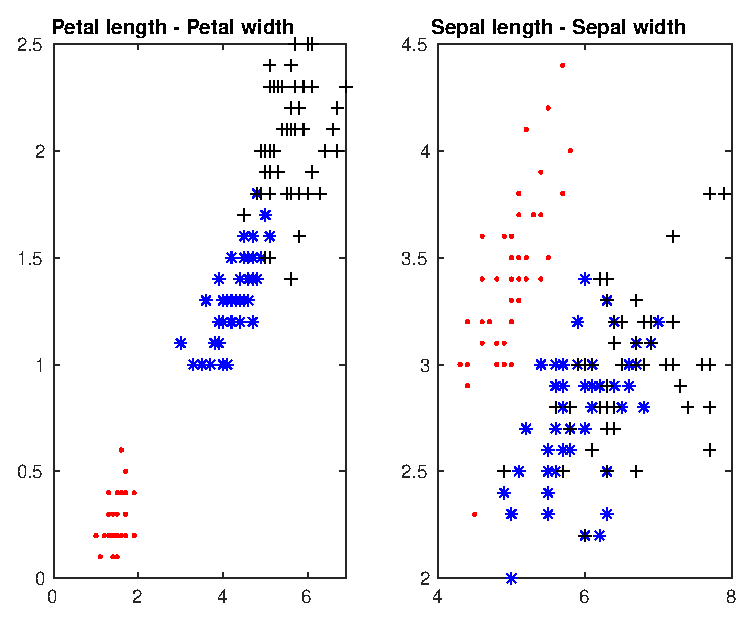
\includegraphics[width=\textwidth]{dataset}
 \caption{Data clusters}
 \label{fig: dataset}
\end{figure}


\section{Gaussian Distributions}

The behaviour of all quantitative traits of the dataset is assumed to adhere to a
Gaussian Distribution.
This assumption is taken due to how the values of the data set are presented.
As shown in Figures
% \ref{fig: sepal length normal distribution},
% \ref{fig: sepal width normal distribution},
\ref{fig: petal length normal distribution} and
\ref{fig: petal width normal distribution}
the distribution for each flower variety follows the
general behaviour of the Gaussian Distribution.

Having confirmed that all quantitative features of the dataset
adhere to Gaussian Distributions, it is possible to proceed with the
development of the classifiers.

% \begin{figure}[htb!]
%  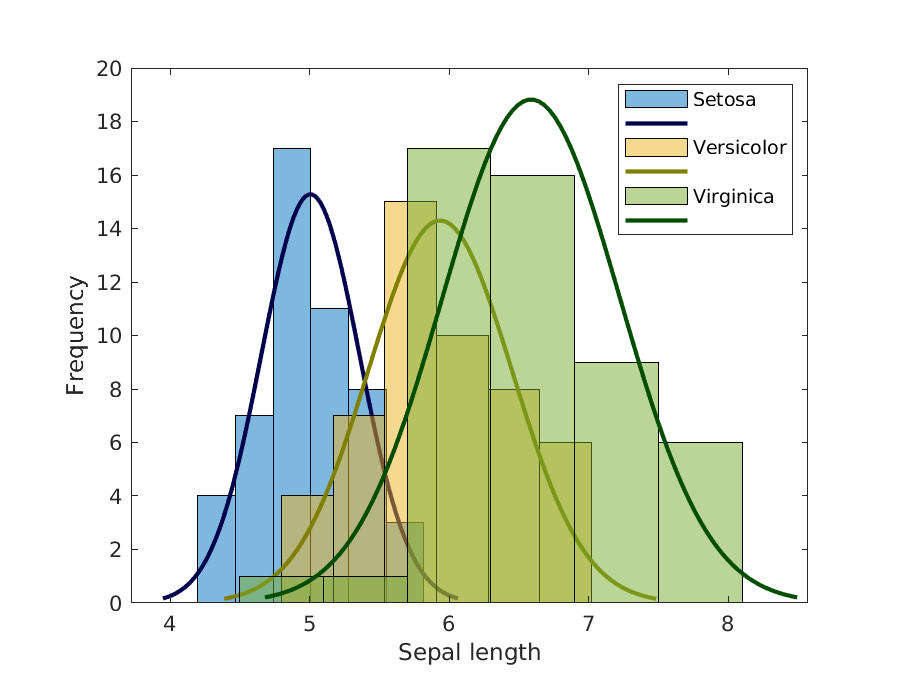
\includegraphics[width=\textwidth]{normSepalLength}
%  \caption{Sepal Length}
%  \label{fig: sepal length normal distribution}
% \end{figure}
%
% \begin{figure}[htb!]
%  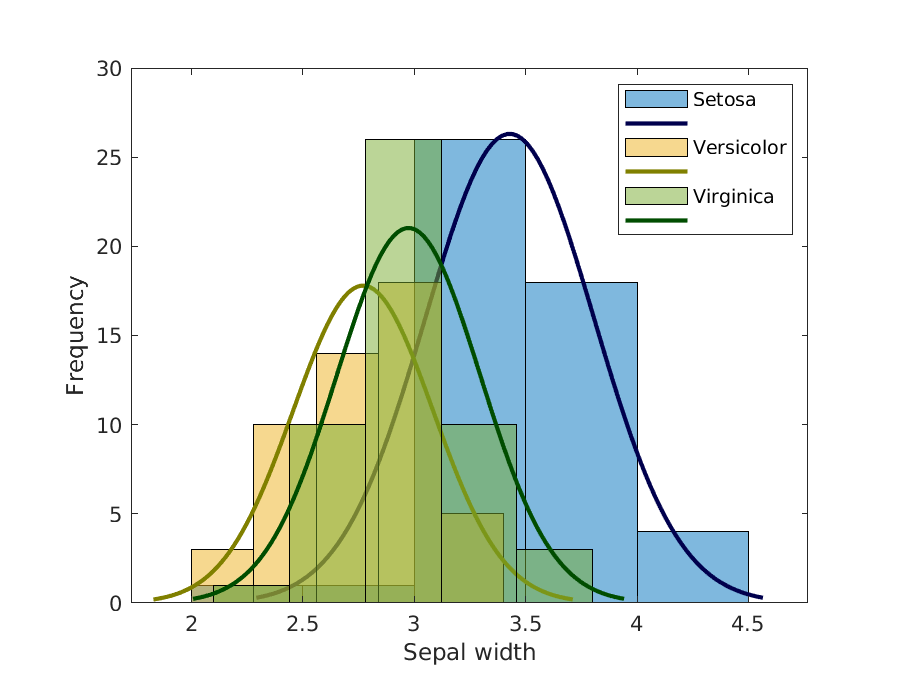
\includegraphics[width=\textwidth]{normSepalWidth}
%  \caption{Sepal Width}
%  \label{fig: sepal width normal distribution}
% \end{figure}

\begin{figure}[htb!]
 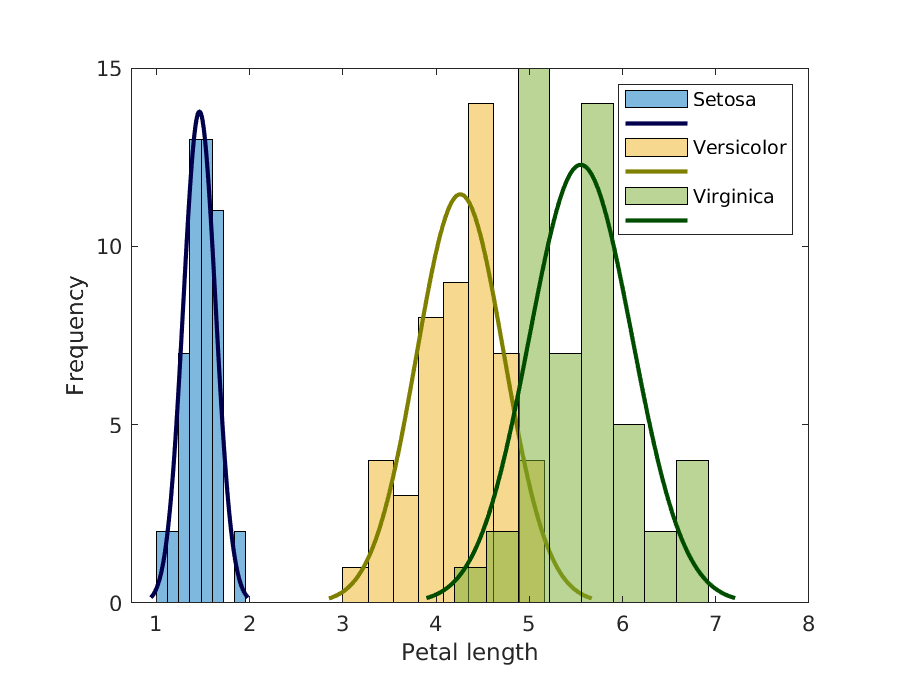
\includegraphics[width=\textwidth]{normPetalLength}
 \caption{Petal Length}
 \label{fig: petal length normal distribution}
\end{figure}

\begin{figure}[htb!]
 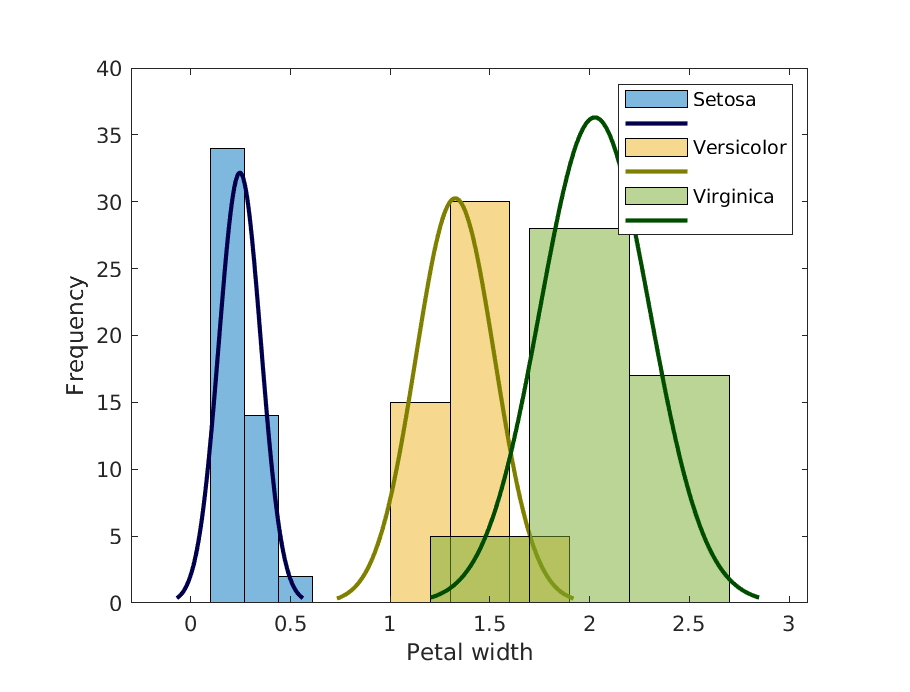
\includegraphics[width=\textwidth]{normPetalWidth}
 \caption{Petal Width}
 \label{fig: petal width normal distribution}
\end{figure}



\pagebreak
\newpage

\pagebreak
\newpage

\pagebreak
\newpage

\section{Classifier}

Classifiers were developed for three cases.

\begin{itemize}
 \item Classifier with $\Sigma = \sigma^2 \cdot \mathbf{I}$
 \item Classifier with $\Sigma = \Sigma_i$
 \item Classifier with arbitrary $\Sigma$
\end{itemize}


\subsection{Case A}
For the first case, $\sigma$ was assigned as $\sigma = 0.25$.
Given this restriction, the multivariate PDF was obtained, as shown in Figure \ref{fig: case a PDF}

\begin{figure}[htb!]
\centering
 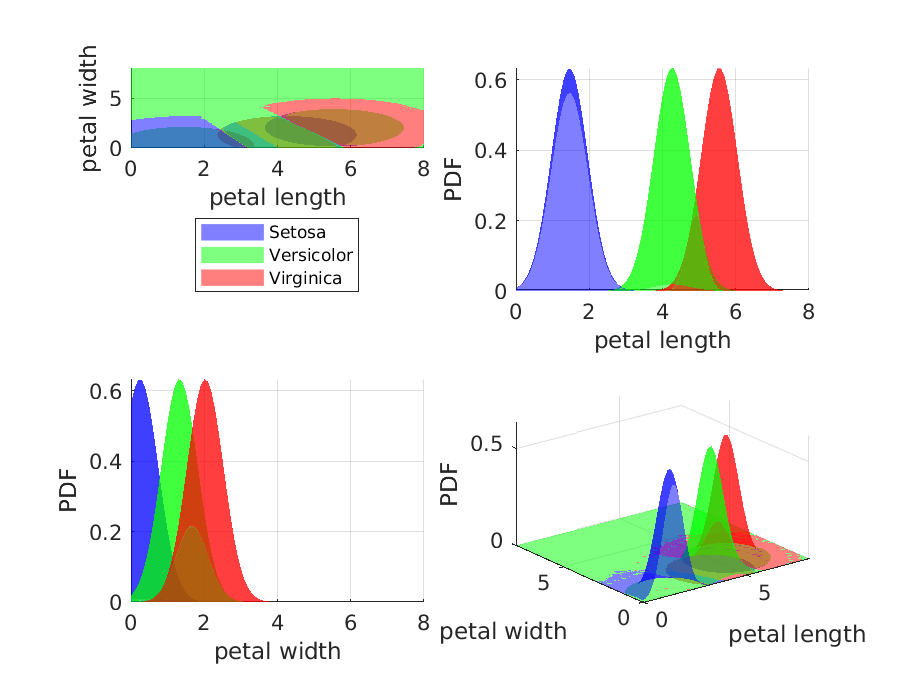
\includegraphics[width = 0.8\textwidth]{pdfCaseA}
 \caption{PDF for Case A}
 \label{fig: case a PDF}
\end{figure}

\begin{align*}
 g_i(x) &= - \frac{\norm{x-\mu_i}^2}{2\sigma^2} + \ln P(\omega_i)\\
 \norm{x-\mu_i}^2 &= (x-\mu_i)^T (x-\mu_i)\\
 g_i(x) &= w^T_i x + \omega_{i0}\\
 w_i &= \frac{1}{\sigma^2} \mu\\
 w_{i0} &= \frac{-1}{2 \sigma^2} \mu^T_i \mu_i + ļn P(\omega_i)
\end{align*}


\pagebreak
\newpage


Afterwards, the \emph{a posteriori} probability is obtained and the boundaries of the classifier are obtained.
The results are shown in Figure \ref{fig: posteriori case A}.

\begin{figure}[htb!]
\centering
 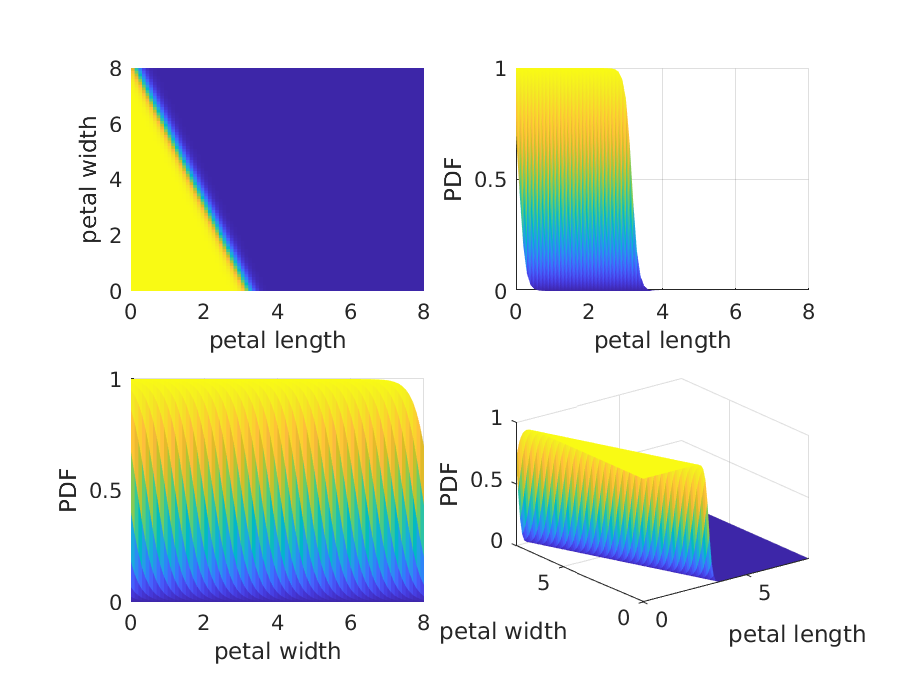
\includegraphics[width= 0.8\textwidth]{classifierSetosaCaseA}
 \caption{Case A - A posteriori probability}
 \label{fig: posteriori case A}
\end{figure}




\pagebreak
\newpage


The classifier was tested against a sample of 75 entries from the dataset. Each entry was assigned a colour based on the assigned variety:
yellow for Setosa, black for Versicolor and magenta for Virginica.
This is presented in Figure \ref{fig: classifier case A}.

\begin{figure}[htb!]
\centering
 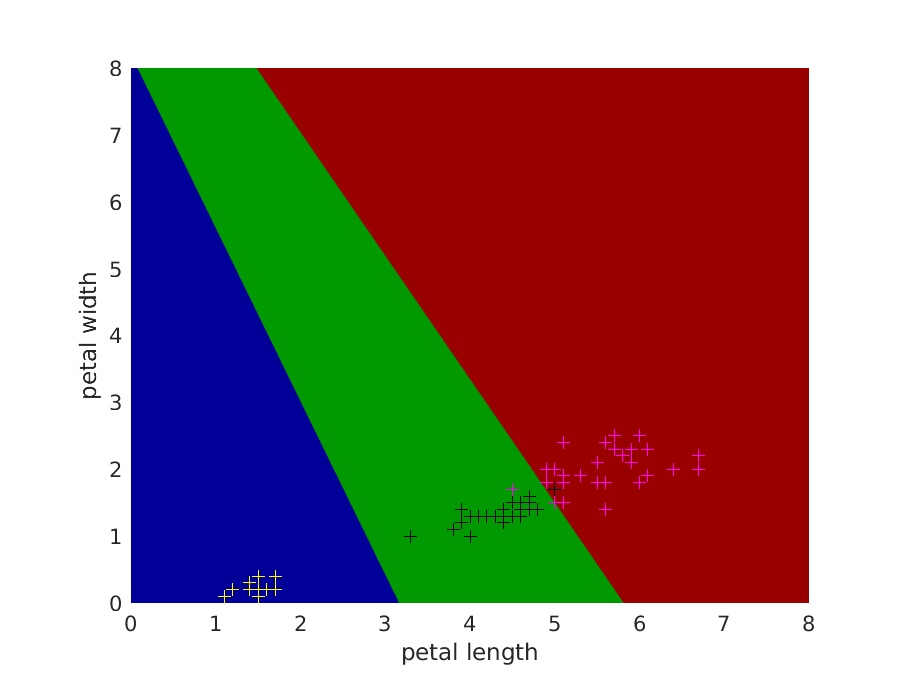
\includegraphics[width= \textwidth]{testClassifierCaseA}
 \caption{Case A - Boundaries}
 \label{fig: classifier case A}
\end{figure}




\pagebreak
\newpage

\pagebreak
\newpage

\subsection{Case B}
For the first case, $\Sigma$ was assigned as

\begin{equation*}
 \begin{pmatrix}
  0.26 & 0.04 &  0.02 & 0.01 \\
  0.04 &  0.22 & 0.03 & 0.02 \\
  0.02 & 0.03 & 0.15 & 0.15\\
  0.01 & 0.02 &  0.15 & 0.31
 \end{pmatrix}
\end{equation*}

This new covariance matrix influenced the multivariate gaussian distribution of the system,
as seen in Figure \ref{fig: case b PDF}.

\begin{figure}[htb!]
 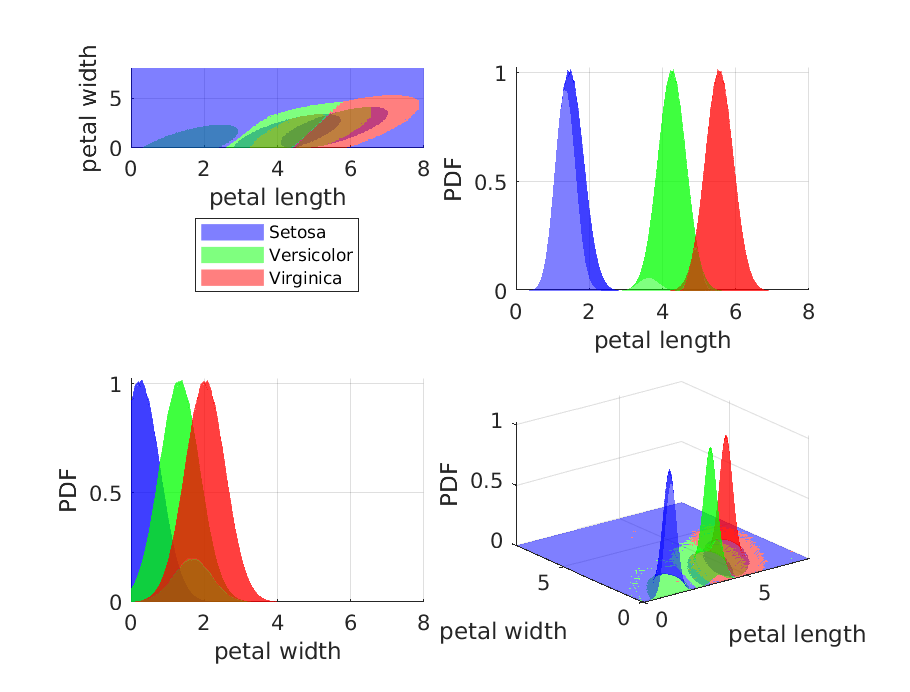
\includegraphics[width = \textwidth]{pdfCaseB}
 \caption{PDF for Case B}
 \label{fig: case b PDF}
\end{figure}

\pagebreak
\newpage


Afterwards, the \emph{a posteriori} probability is obtained and the boundaries of the classifier are obtained.
The results are shown in Figure \ref{fig: posteriori case B}.

\begin{figure}[htb!]
\centering
 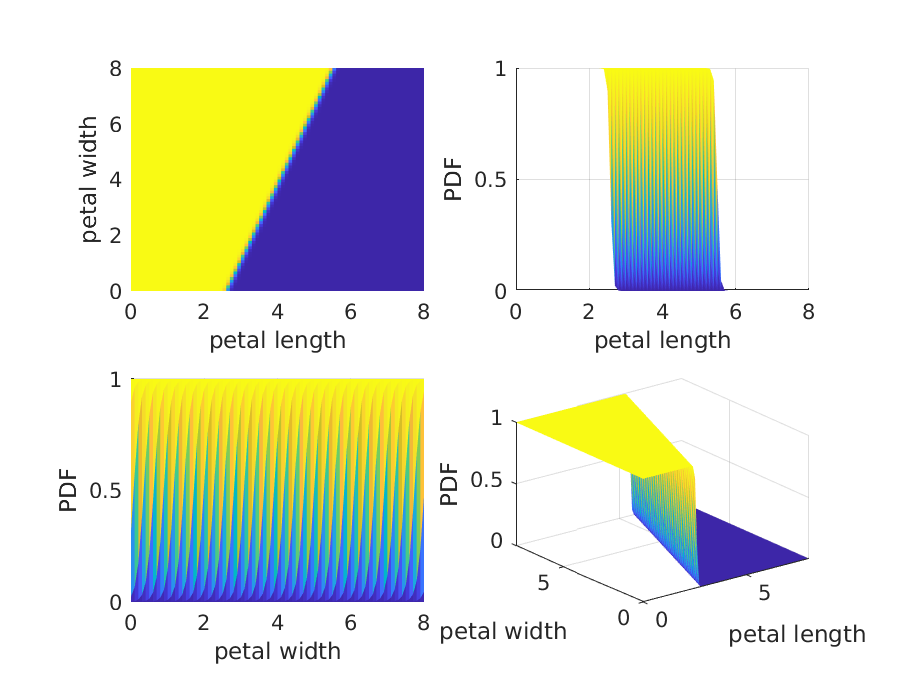
\includegraphics[width= 0.8\textwidth]{classifierSetosaCaseB}
 \caption{Case B - A posteriori probability}
 \label{fig: posteriori case B}
\end{figure}

\begin{align*}
 g_i(x) &= x^T W_i x + w^T_i x + \omega_{i0}\\
 W_i &= -\frac{1}{2}\Sigma^{-1}_i\\
 w_i &= \Sigma^{-1}_i \mu_i\\
 \omega_{i0}&= -\frac{1}{2} \mu^T_i \Sigma^{-1}_i \mu_i - \frac{1}{2}\ln \det(\Sigma_i) + \ln P(\omega_i)
\end{align*}

\pagebreak
\newpage


The classifier was tested against a sample of 75 entries from the dataset. Each entry was assigned a colour based on the assigned variety:
yellow for Setosa, black for Versicolor and magenta for Virginica.
This is presented in Figure \ref{fig: classifier case B}.

\begin{figure}[htb!]
\centering
 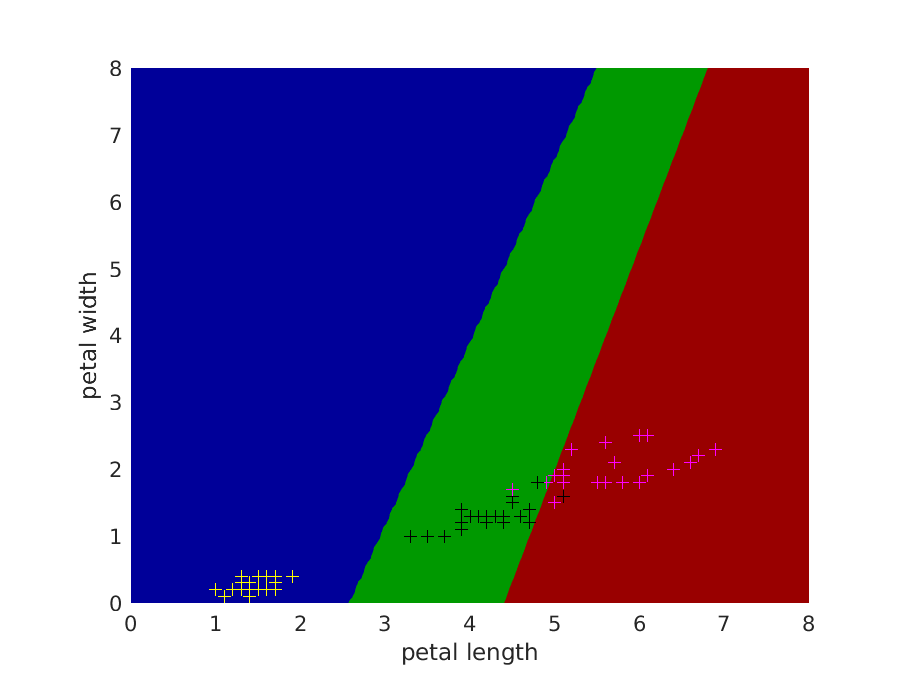
\includegraphics[width= \textwidth]{testClassifierCaseB}
 \caption{Case B - Boundaries}
 \label{fig: classifier case B}
\end{figure}

\pagebreak
\newpage


\pagebreak
\newpage

\subsection{Case C}
For the third case, $\Sigma$ was left untouched, allowing the covariance matrix to
reflect the nature of the data available.
This is observed in Figure \ref{fig: case c PDF}.

\begin{figure}[htb!]
 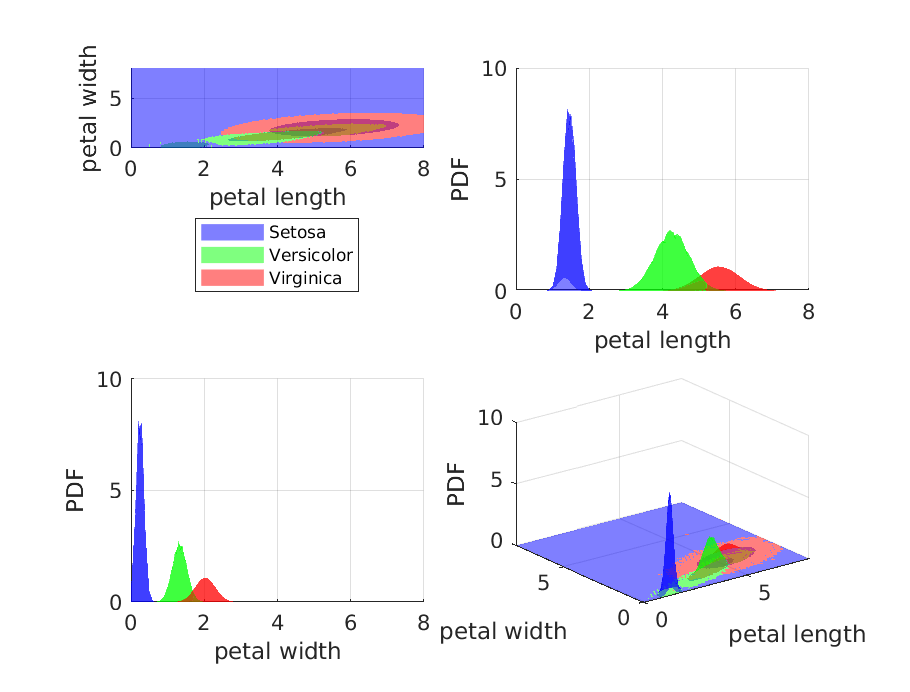
\includegraphics[width = \textwidth]{pdfCaseC}
 \caption{PDF for Case C}
 \label{fig: case c PDF}
\end{figure}

\pagebreak
\newpage


Afterwards, the \emph{a posteriori} probability is obtained and the boundaries of the classifier are obtained.
The results are shown in Figure \ref{fig: posteriori case C}.

\begin{figure}[htb!]
\centering
 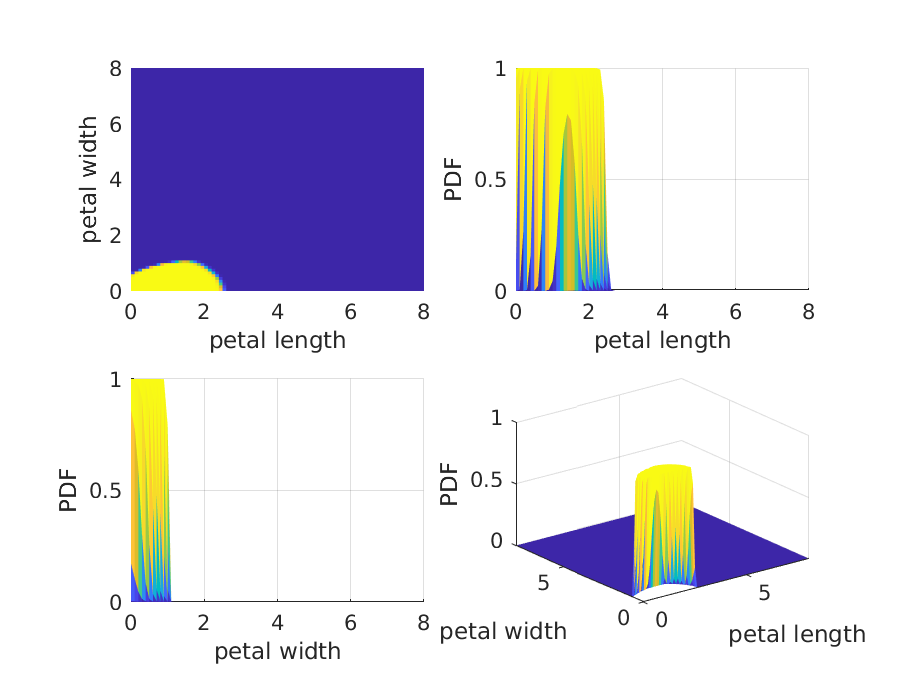
\includegraphics[width= 0.8\textwidth]{classifierSetosaCaseC}
 \caption{Case C - A posteriori probability}
 \label{fig: posteriori case C}
\end{figure}

\pagebreak
\newpage

\begin{align*}
 g_i(x) &= -\frac{1}{2} (x-\mu_i)^T \Sigma^{-1} (x-\mu) + \ln P(\omega_i)\\
 g_i(x) &= w^T_i x + \omega_{i0}\\
 w_i &= \Sigma^{-1} \mu_i\\
 w_{i0} &= \frac{-1}{2}\mu^T_i \Sigma^{-1}  \mu_i + ļn P(\omega_i)
\end{align*}

The classifier was tested against a sample of 75 entries from the dataset. Each entry was assigned a colour based on the assigned variety:
yellow for Setosa, black for Versicolor and magenta for Virginica.
This is presented in Figure \ref{fig: classifier case C}.

\begin{figure}[htb!]
\centering
 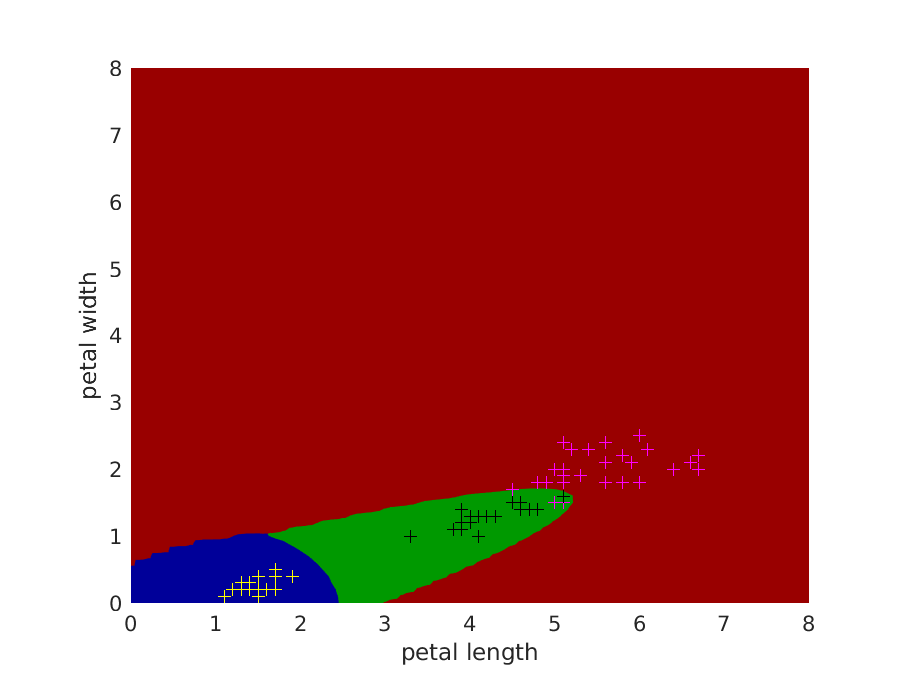
\includegraphics[width= \textwidth]{testClassifierCaseC}
 \caption{Case C - Boundaries}
 \label{fig: classifier case C}
\end{figure}

\pagebreak
\newpage

\section{Errors}

The error boundaries for the classifiers were obtained
for both the Chernoff and Bhattacharyya Bounds \cite{duda2012pattern}.

For the Chernoff Bounds, the following equations were employed.

\begin{align*}
 \min[a,b] & \leq a^\beta b^{1-\beta}  \quad \text{for } a,b \geq 0 \text{ and } 0\leq \beta \leq 1  \\
 P(\text{error}) & \leq P^\beta (\omega_1) P^{1-\beta} (\omega_2) \int p^\beta (x | \omega_1)p^{1-\beta}(x|\omega_2)dx  \text{ for } 0 \leq \beta \leq 1\\
\int p^\beta &(x | \omega_1)p^{1-\beta}(x|\omega_2)dx  = \exp(-k(\beta)) \\
k(\beta) &= \frac{\beta(1-\beta)}{2} (\mu_2 - \mu_1)^T \det(\beta  \Sigma_1 + (1-\beta)\Sigma_2)^{-1} (\mu_2 - \mu_1) \\
& \quad + \frac{1}{2} \ln \frac{\det(\beta \Sigma_1  + (1-\beta)\Sigma_2)}{\det(\Sigma_1)^\beta \det(\Sigma_2)^{1-\beta}}
 \end{align*}

 Likewise, for the Bhattacharyya Bounds another set of equations was utilized

\begin{align*}
 P(\text{error}) & \leq \sqrt{P{\omega_1} P(\omega_2)} \int \sqrt{p(x | \omega_1) p(x|\omega_2)} dx\\
 &= \sqrt{P{\omega_1} P(\omega_2)} \exp{-k(1/2)}\\
 k(1/2) &= \frac{1}{8}(\mu_2 - \mu_1)^T \det(\frac{\Sigma_1 + Sigma_2}{2})^{-1} (\mu_2 + mu_1) \\
 & \quad + \frac{1}{2} \ln \frac{\det(\frac{\Sigma_1 + \Sigma_2}{2})}{\sqrt{\det(\Sigma_1)\det(\Sigma_2)}}
\end{align*}


\subsection{Case A}

For this case, the Chernoff bounds were determined to be

\begin{table}[htb]
\begin{center}
\begin{tabular}{ll}
$P_{12}$ & 0.3712\%\\
$P_{23}$ & 11.3240\%\\
$P_{31}$ & 0.0016\%
\end{tabular}
\end{center}
\caption{Case A - Chernoff Bound}
\label{tab: case a chernoff}
\end{table}

Likewise the Bhattacharyya bounds were determined


\begin{table}[htb]
\begin{center}
\begin{tabular}{ll}
$P_{12}$ & 0.3712\%\\
$P_{23}$ & 11.3240\%\\
$P_{31}$ & 0.0016\%
\end{tabular}
\end{center}
\caption{Case A - Bhattacharyya Bound}
\label{tab: case a bhatt}
\end{table}

\begin{figure}
 \centering
 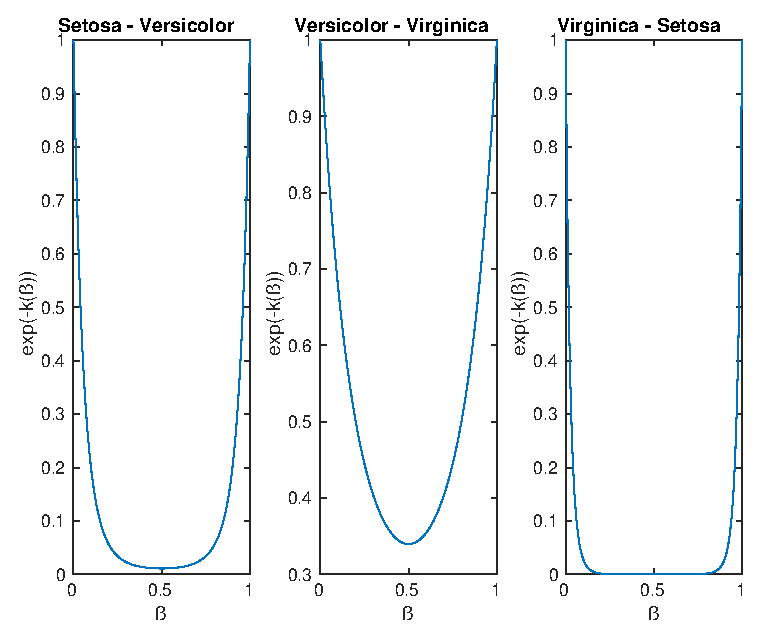
\includegraphics{errorCaseA}
 \caption{Case A - Error bound}
 \label{case a error}
\end{figure}

The experimental error was also examined for the data set.

\begin{table}[htb]
\begin{center}
\begin{tabular}{ll}
$P_{12}$ & 0.000\%\\
$P_{23}$ & 4.000\%\\
$P_{31}$ & 0.000\%
\end{tabular}
\end{center}
\caption{Case A - Experimental error}
\label{tab: case a experiment}
\end{table}


% errorExp =
%
%          0    0.0400         0

\newpage
\pagebreak

\subsection{Case B}

For this case, the Chernoff bounds were determined to be

\begin{table}[htb]
\begin{center}
\begin{tabular}{ll}
$P_{12}$ & 0.0049\%\\
$P_{23}$ & 6.3073\%\\
$P_{31}$ & 0.0000\%
\end{tabular}
\end{center}
\caption{Case B - Chernoff Bound}
\label{tab: case b chernoff}
\end{table}

Likewise the Bhattacharyya bounds were determined


\begin{table}[htb!]
\begin{center}
\begin{tabular}{ll}
$P_{12}$ & 0.0049\%\\
$P_{23}$ & 6.3073\%\\
$P_{31}$ & 0.0000
\end{tabular}
\end{center}
\caption{Case B - Bhattacharyya Bound}
\label{tab: case b bhatt}
\end{table}


\begin{figure}
 \centering
 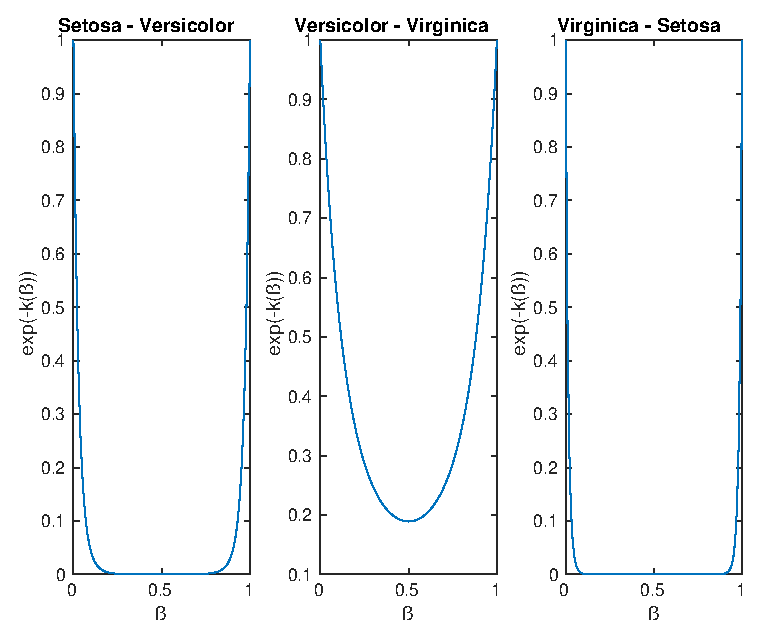
\includegraphics{errorCaseB}
 \caption{Case B - Error bound}
 \label{case b error}
\end{figure}


The experimental error was also examined for the data set.

\begin{table}[htb]
\begin{center}
\begin{tabular}{ll}
$P_{12}$ & 0.000\%\\
$P_{23}$ & 8.000\%\\
$P_{31}$ & 0.000\%
\end{tabular}
\end{center}
\caption{Case B - Experimental error}
\label{tab: case b experiment}
\end{table}

% errorExp =
%
%          0    0.0800         0

\newpage
\pagebreak

\subsection{Case C}

For this case, the Chernoff bounds were determined to be

\begin{table}[htb!]
\begin{center}
\begin{tabular}{ll}
$P_{12}$ & 0.0012\%\\
$P_{23}$ & 7.9909\%\\
$P_{31}$ & 0.0000\%
\end{tabular}
\end{center}
\caption{Case C - Chernoff Bound}
\label{tab: case c chernoff}
\end{table}

Likewise the Bhattacharyya bounds were determined


\begin{table}[htb!]
\begin{center}
\begin{tabular}{ll}
$P_{12}$ & 0.0074\%\\
$P_{23}$ & 8.0726\%\\
$P_{31}$ & 0.0000\%
\end{tabular}
\end{center}
\caption{Case C - Bhattacharyya Bound}
\label{tab: case c bhatt}
\end{table}

\begin{figure}
 \centering
 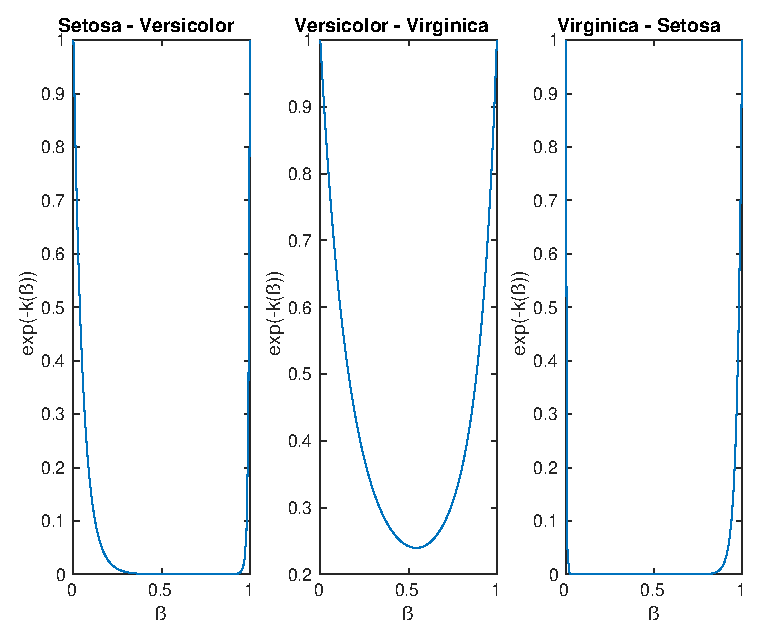
\includegraphics{errorCaseC}
 \caption{Case C - Error bound}
 \label{case c error}
\end{figure}

The experimental error was also examined for the data set.

\begin{table}[htb]
\begin{center}
\begin{tabular}{ll}
$P_{12}$ & 0.000\%\\
$P_{23}$ & 3.333\%\\
$P_{31}$ & 0.000\%
\end{tabular}
\end{center}
\caption{Case C - Experimental error}
\label{tab: case c experiment}
\end{table}


% errorExp =
%
%          0    0.0333         0


\newpage
\pagebreak
\printbibliography

% \newpage
% \pagebreak
% \appendix
% \section{Octave Code}
% \lstinputlisting[language=Matlab]{<filename>.m}

\end{document}
